\definecolor{r1}{RGB}{86,16,16};
\definecolor{r2}{RGB}{151,28,28};
\definecolor{r3}{RGB}{214,39,40};
\definecolor{r4}{RGB}{227,104,104};
\definecolor{r5}{RGB}{239,169,169};
\definecolor{b1}{RGB}{11,43,65};
\definecolor{b2}{RGB}{22,86,131};
\definecolor{b3}{RGB}{31,119,180};
\definecolor{b4}{RGB}{59,154,222};
\definecolor{b5}{RGB}{124,188,233};
\definecolor{g1}{RGB}{16,60,16};
\definecolor{g2}{RGB}{33,120,33};
\definecolor{g3}{RGB}{49,180,49};
\definecolor{g4}{RGB}{95,211,95};
\definecolor{g5}{RGB}{135,222,135};
\definecolor{p1}{RGB}{39,23,53};
\definecolor{p2}{RGB}{77,47,106};
\definecolor{p3}{RGB}{116,70,160};
\definecolor{p4}{RGB}{148,103,189};
\definecolor{p5}{RGB}{179,149,208};
\definecolor{tab_orange}{RGB}{255,127,14};
\definecolor{tab_blue}{RGB}{31, 119, 180};
\definecolor{mixed_color}{RGB}{143, 123, 97}
\definecolor{tab_brown}{RGB}{140,86,75};


\begin{tikzpicture}


\node at (9.1,15.8) {{\fontfamily{phv}\scalebox{1}{\fontsize{12pt}{0pt}\selectfont{A2}}}};
\node at (13.6,15.8) {{\fontfamily{phv}\scalebox{1}{\fontsize{8pt}{0pt}\selectfont \parbox{8cm} {\hyphenpenalty=10000\exhyphenpenalty=10000\raggedright Coronal view of CVR maps from GMV models trained with PPND SSD sample }}}};
\node[inner sep=0pt] (russell) at (11.6,11.5) {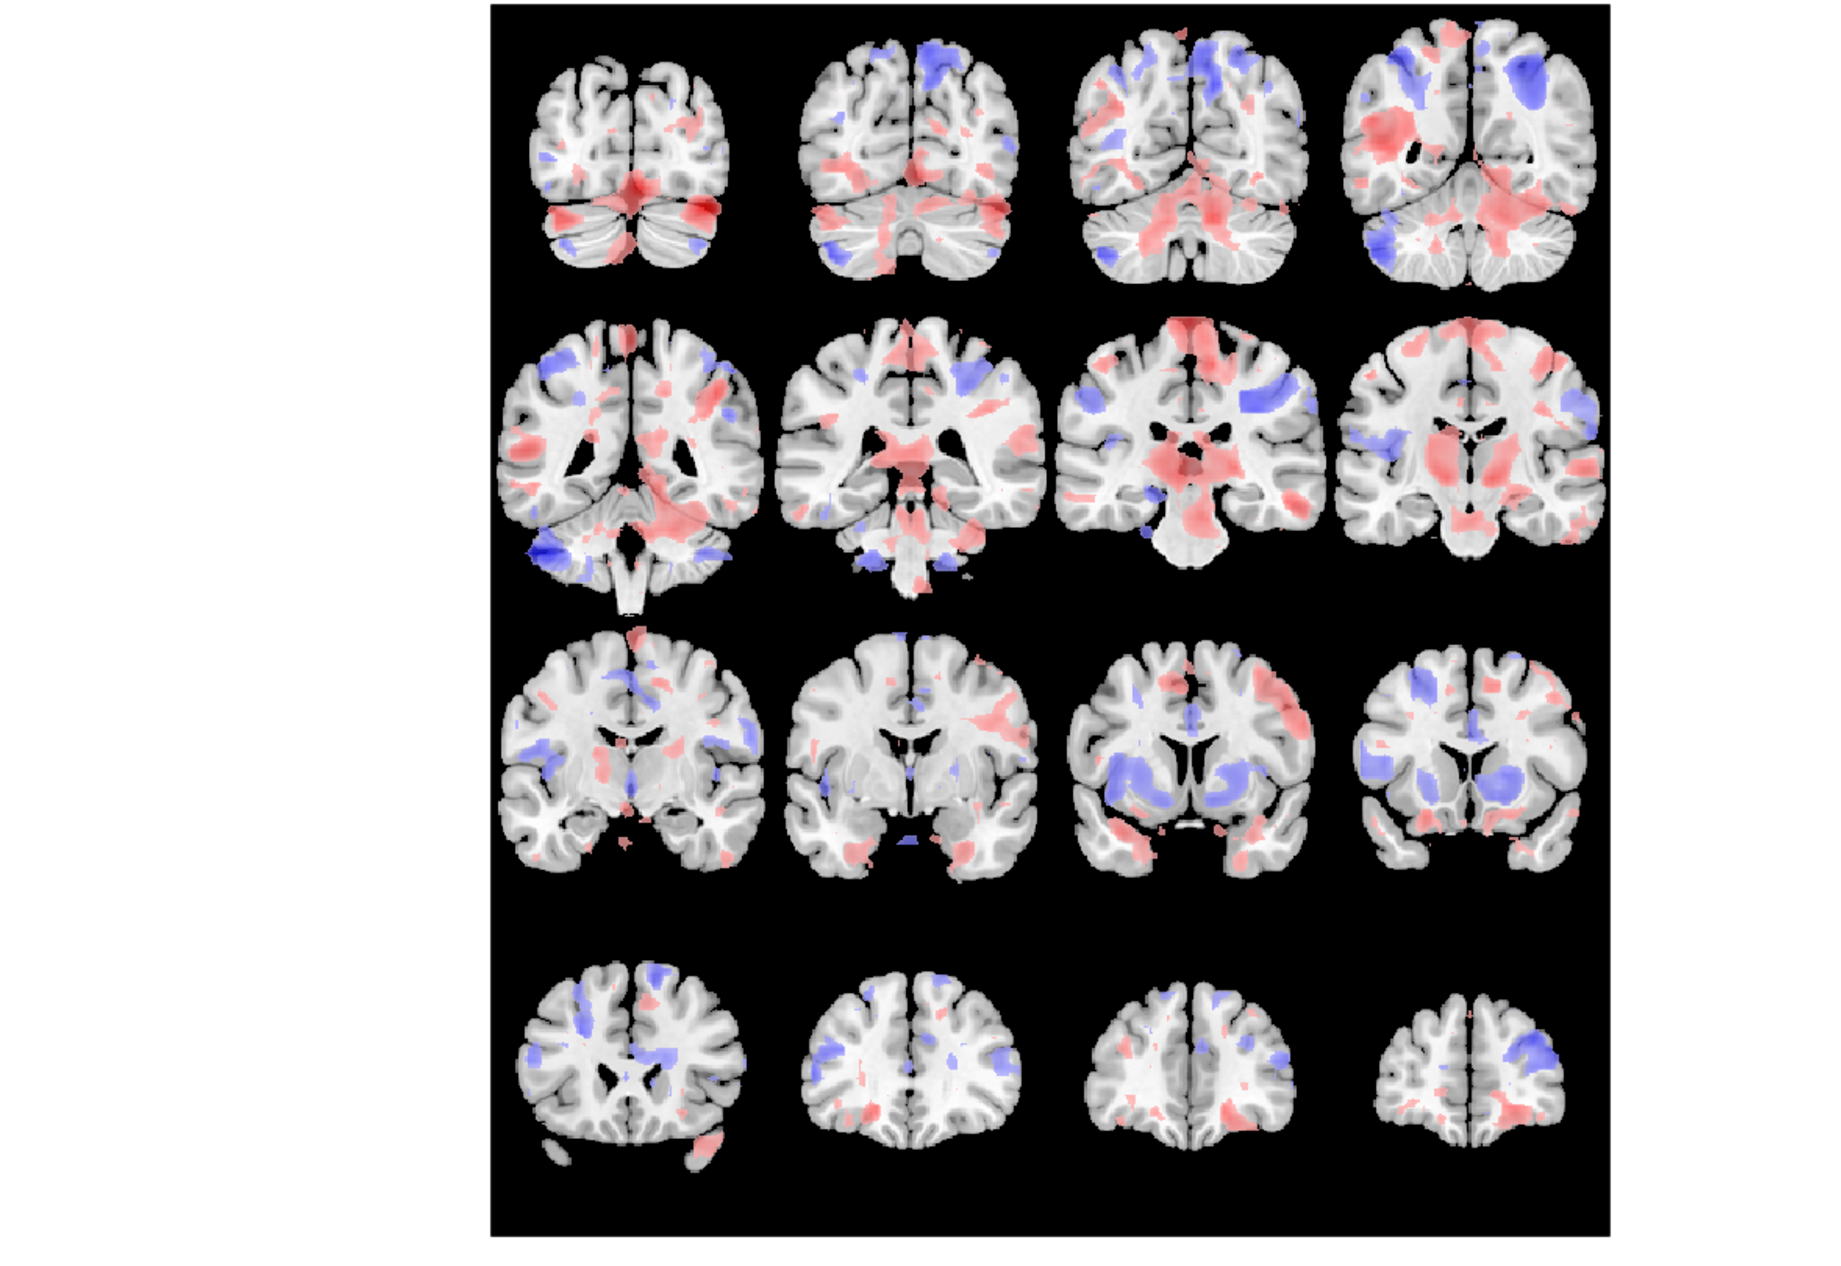
\includegraphics[width=0.50\textwidth]{dpsdi_mwp1_coronal.pdf}};

\node at (-0.3,15.8) {{\fontfamily{phv}\scalebox{1}{\fontsize{12pt}{0pt}\selectfont{A1}}}};
\node at (4.2,15.8) {{\fontfamily{phv}\scalebox{1}{\fontsize{8pt}{0pt}\selectfont \parbox{8cm} {\hyphenpenalty=10000\exhyphenpenalty=10000\raggedright Axial view of CVR maps from GMV models trained with PPND SSD sample }}}};
\node[inner sep=0pt] (russell) at (3.45,11.5) {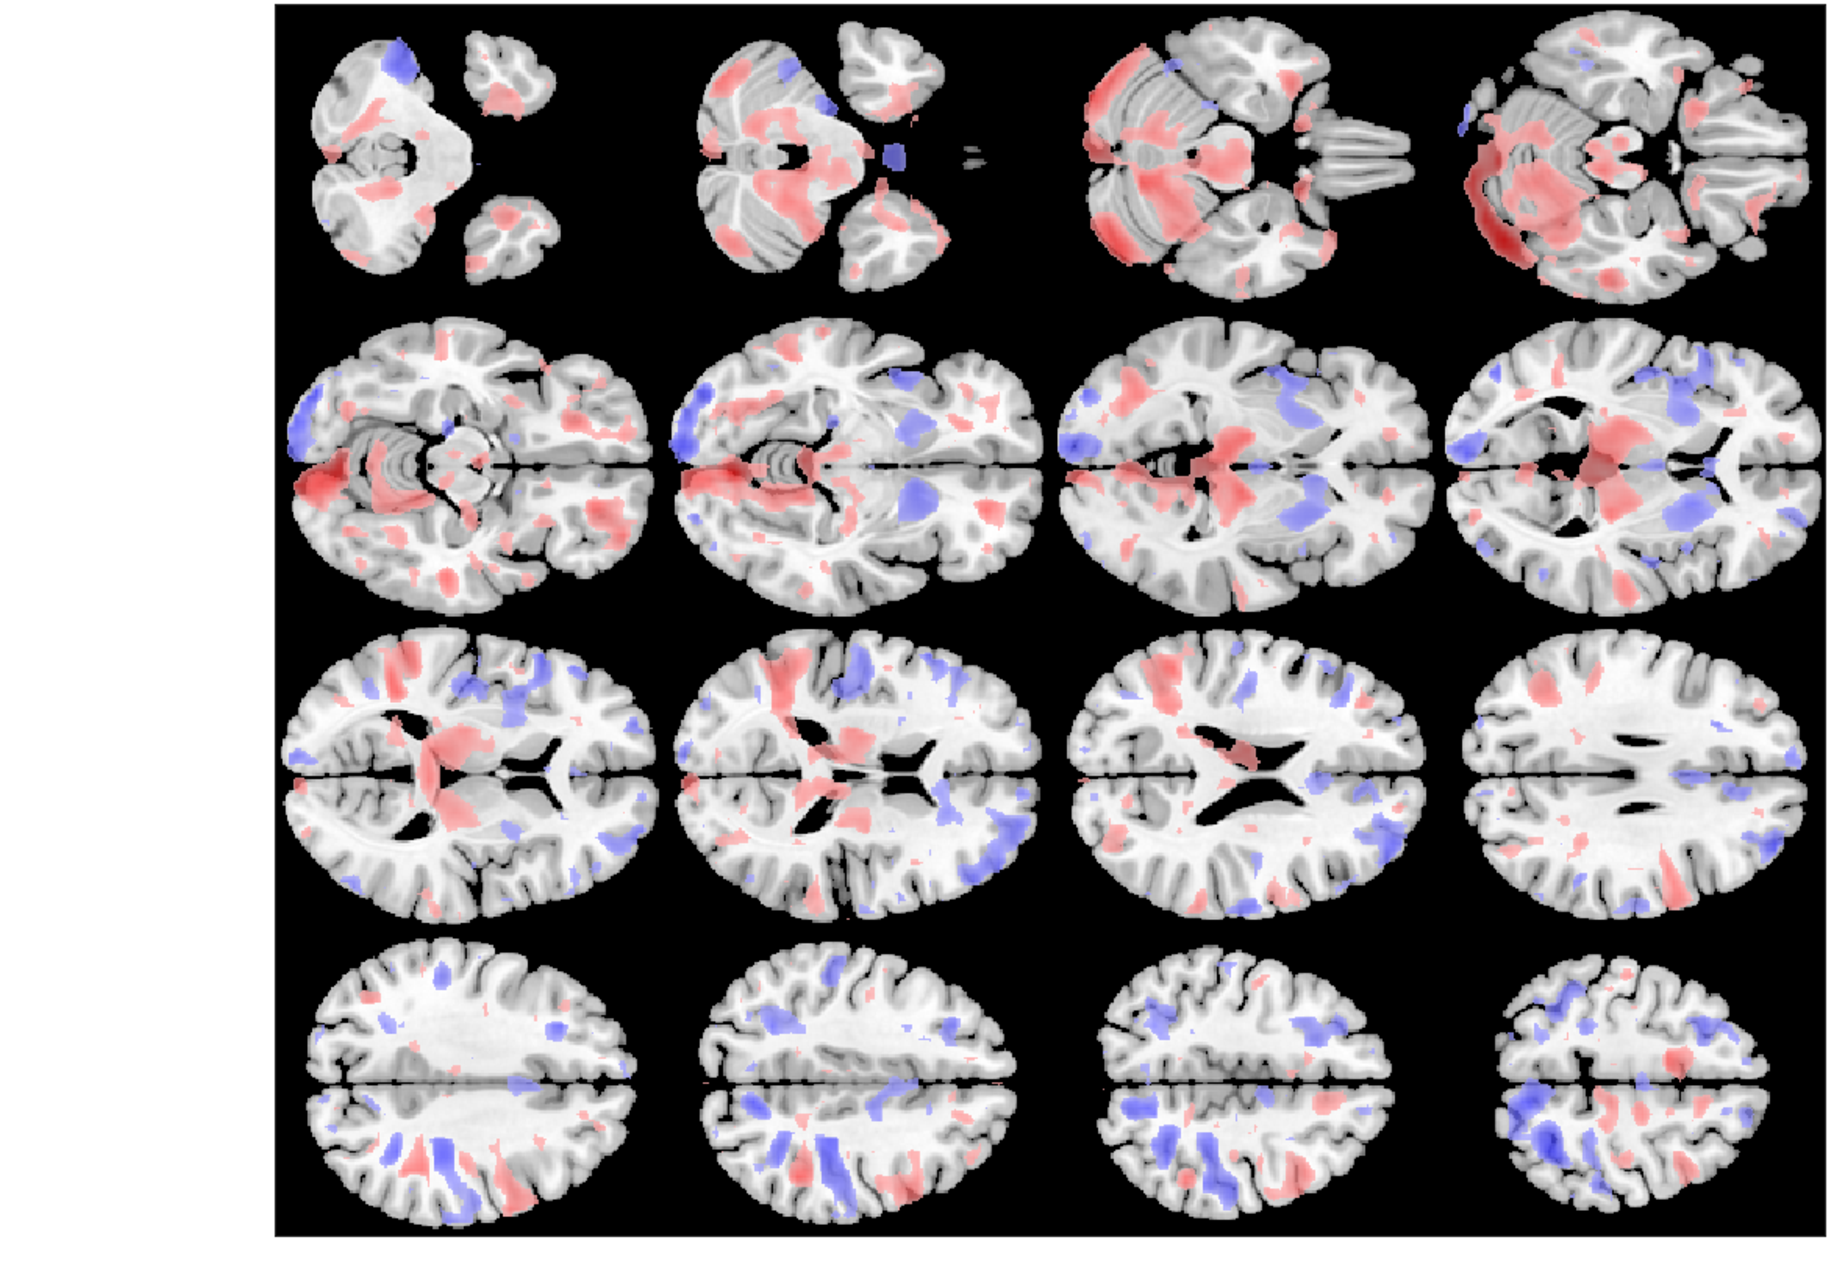
\includegraphics[width=0.50\textwidth]{dpsdi_mwp1_axial.pdf}};

\node[inner sep=0pt] (russell) at (16.46,13.18) {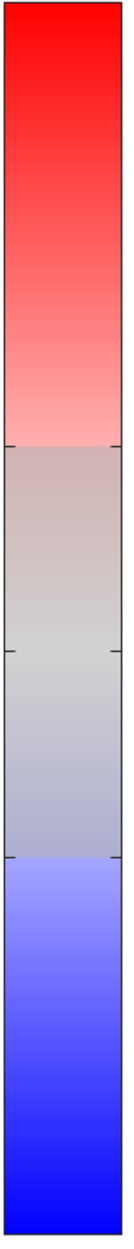
\includegraphics[width=0.02\textwidth]{colorbar.pdf}};



\node at (16.01,15.17) {{\fontfamily{phv}\scalebox{1}{\fontsize{8pt}{0pt}\selectfont{10}}}};
\node at (16.01,13.74) {{\fontfamily{phv}\scalebox{1}{\fontsize{8pt}{0pt}\selectfont{3}}}};
\node at (16.01,12.4) {{\fontfamily{phv}\scalebox{1}{\fontsize{8pt}{0pt}\selectfont{-3}}}};
\node at (16.01,11.2) {{\fontfamily{phv}\scalebox{1}{\fontsize{8pt}{0pt}\selectfont{-10}}}};

\node [rotate = 90] at (16.96,12.9) {{\fontfamily{phv}\scalebox{1}{\fontsize{8pt}{0pt}\selectfont{Cross-validation ratio (CVR)}}}};









\node at (9.1,7) {{\fontfamily{phv}\scalebox{1}{\fontsize{12pt}{0pt}\selectfont{B2}}}};
\node at (13.6,7) {{\fontfamily{phv}\scalebox{1}{\fontsize{8pt}{0pt}\selectfont \parbox{8cm} {\hyphenpenalty=10000\exhyphenpenalty=10000\raggedright Coronal view of CVR maps from GMV models trained with PPND MDD v HC sample }}}};
\node[inner sep=0pt] (russell) at (11.6,2.7) {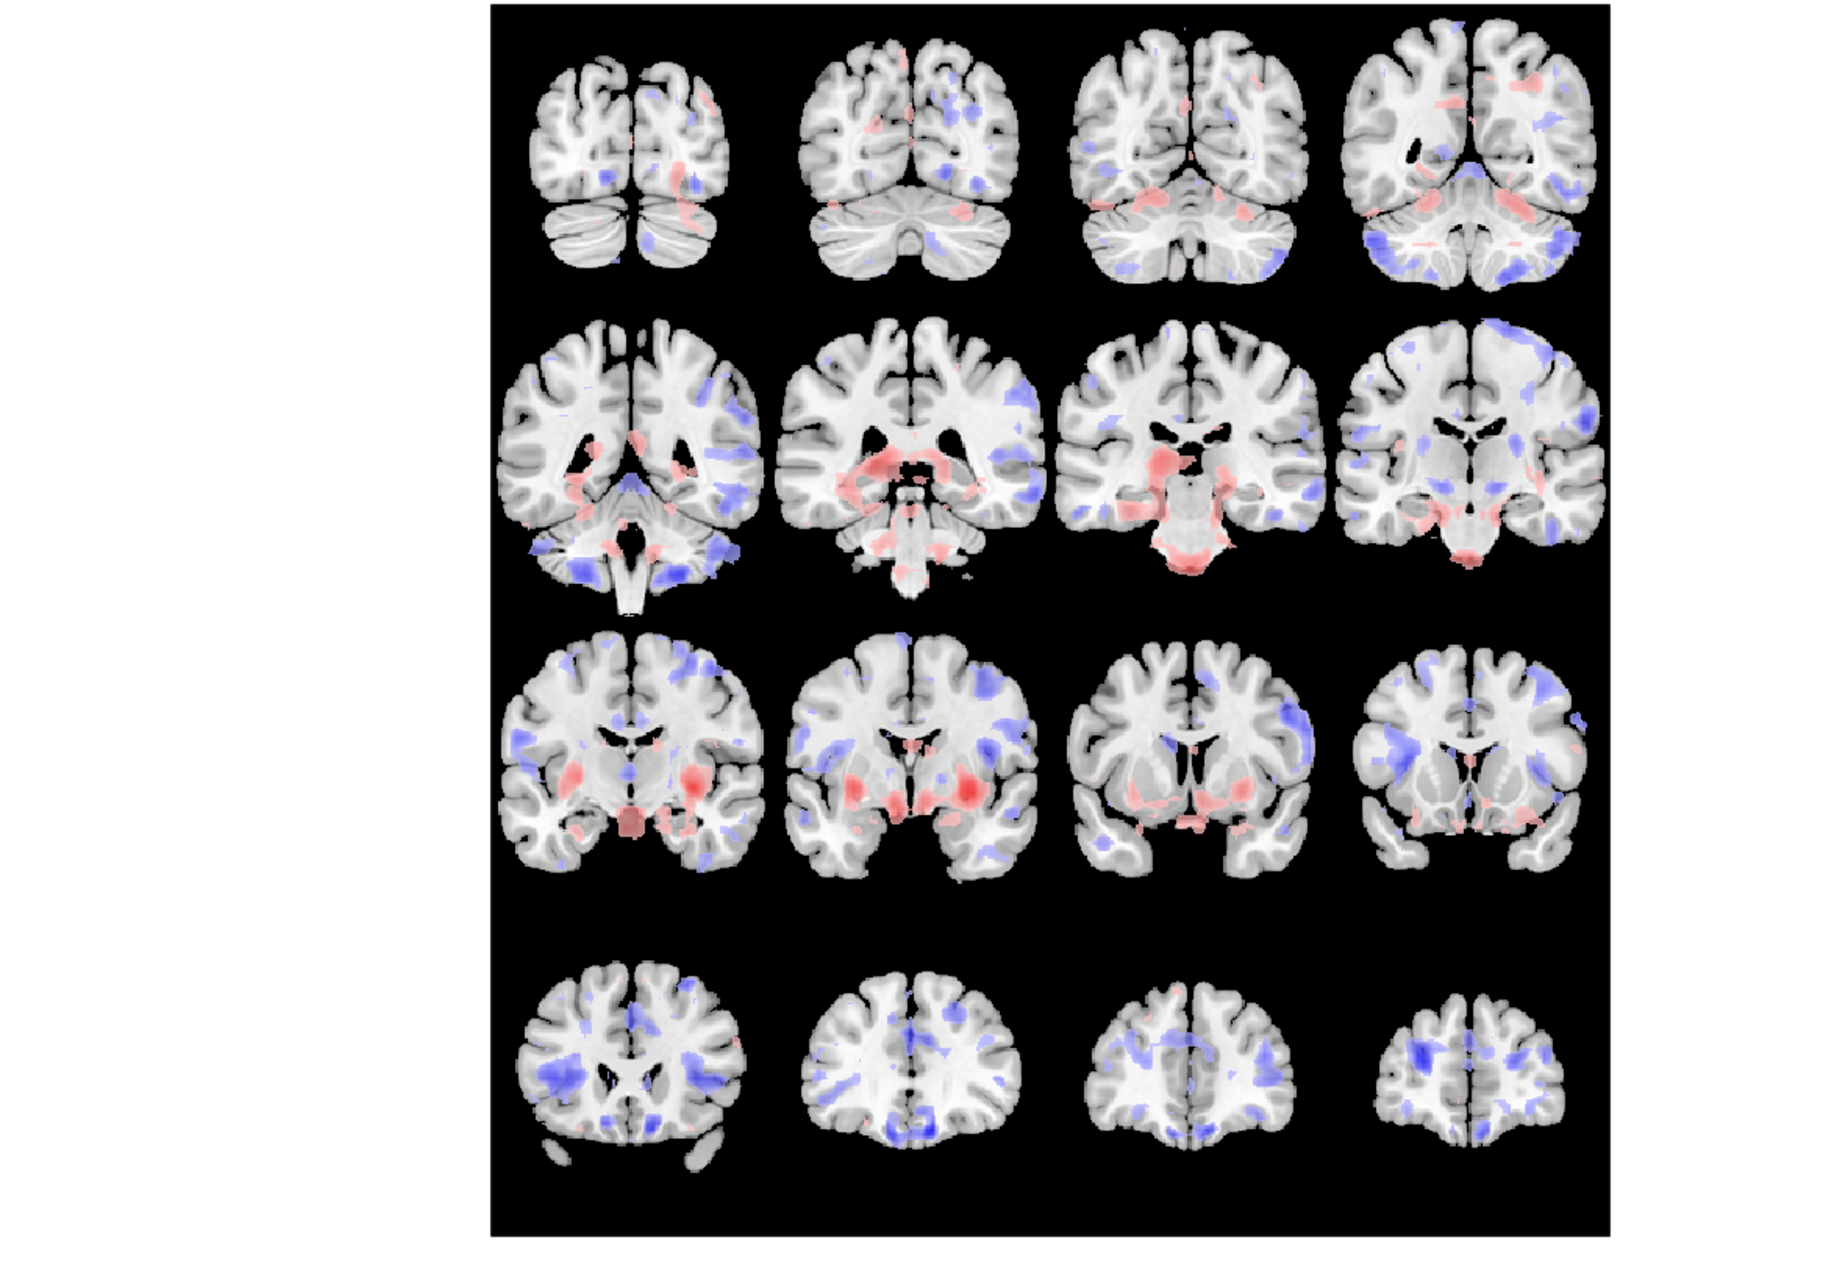
\includegraphics[width=0.50\textwidth]{mdd_mwp1_coronal.pdf}};

\node at (-0.3,7) {{\fontfamily{phv}\scalebox{1}{\fontsize{12pt}{0pt}\selectfont{B1}}}};
\node at (4.2,7) {{\fontfamily{phv}\scalebox{1}{\fontsize{8pt}{0pt}\selectfont \parbox{8cm} {\hyphenpenalty=10000\exhyphenpenalty=10000\raggedright Axial view of CVR maps from GMV models trained with PPND MDD v HC sample }}}};
\node[inner sep=0pt] (russell) at (3.45,2.7) {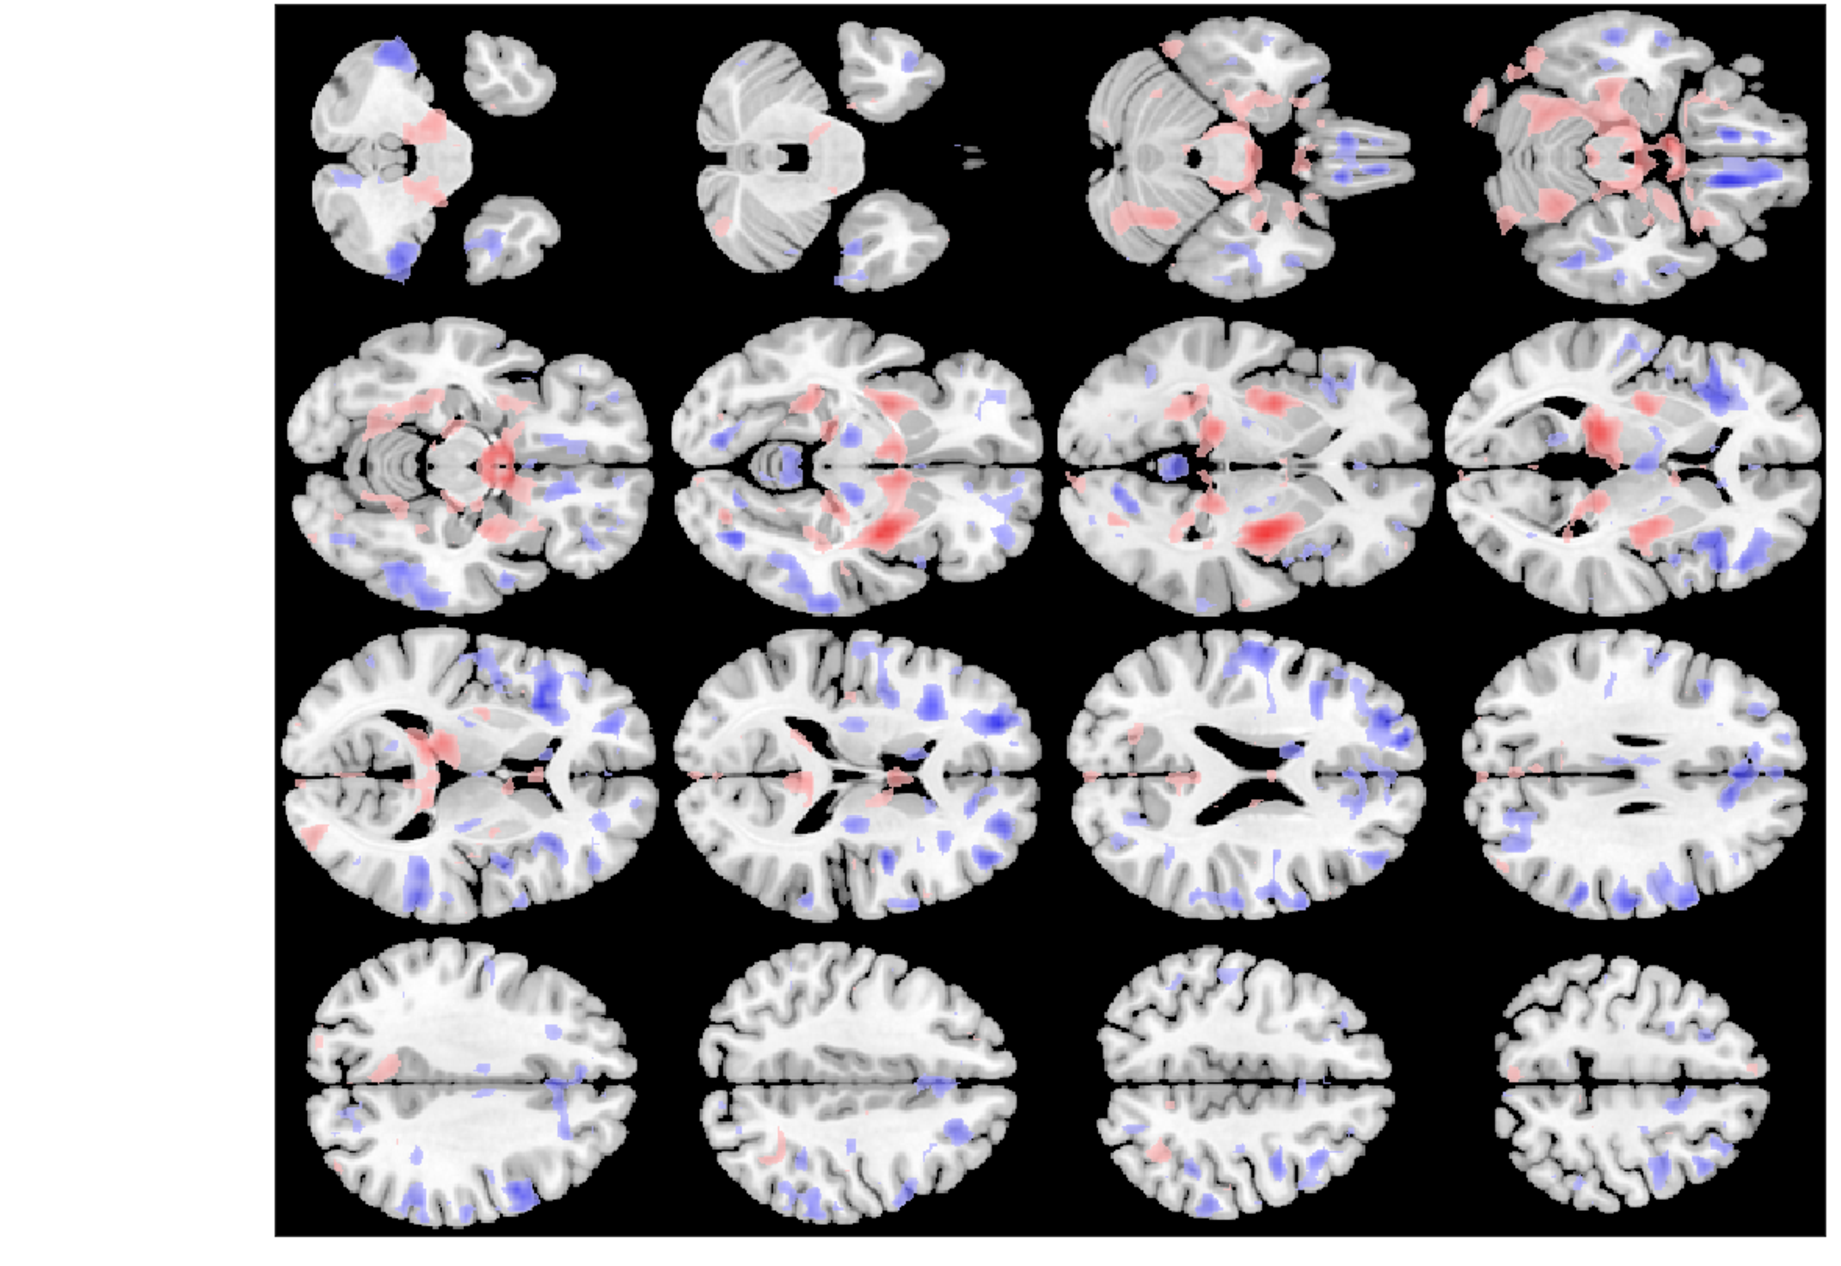
\includegraphics[width=0.50\textwidth]{mdd_mwp1_axial.pdf}};

\node[inner sep=0pt] (russell) at (16.46,4.38) {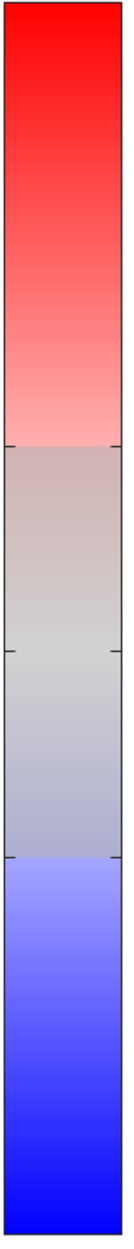
\includegraphics[width=0.02\textwidth]{colorbar.pdf}};



\node at (16.01,6.37) {{\fontfamily{phv}\scalebox{1}{\fontsize{8pt}{0pt}\selectfont{10}}}};
\node at (16.01,4.94) {{\fontfamily{phv}\scalebox{1}{\fontsize{8pt}{0pt}\selectfont{3}}}};
\node at (16.01,3.6) {{\fontfamily{phv}\scalebox{1}{\fontsize{8pt}{0pt}\selectfont{-3}}}};
\node at (16.01,2.4) {{\fontfamily{phv}\scalebox{1}{\fontsize{8pt}{0pt}\selectfont{-10}}}};

\node [rotate = 90] at (16.96,4.1) {{\fontfamily{phv}\scalebox{1}{\fontsize{8pt}{0pt}\selectfont{Cross-validation ratio (CVR)}}}};






























\end{tikzpicture}